\section{Fundamentals of Federated Learning\label{sec:bg.fl}}

Introduced in 2016 by \textcite{mcmahan_Communicationefficientlearningdeep_2017}, \acrfull{fl} changes the usual \gls{ml} paradigm where distributed data is centrally collected, curated, and processed on a dedicated server. 
Instead, \gls{fl} respects the decentralized nature of the data and rather brings model training to the data sources.
By alternating between training on local data and aggregating model updates, \gls{fl} enables the training of a shared model without the need to share the data itself.
This approach reveals itself as a promising solution to multiple challenges faced by traditional \gls{ml} systems.
The two main ones are:
\begin{enumerate}
    \item training models over massively distributed data sources, such as smartphones, wearables, or IoT devices;
    \item training models on sensitive data, such as medical records or financial transactions, while preserving privacy and confidentiality.
\end{enumerate}

Although the term \emph{Federated Learning} was introduced by \textcite{mcmahan_Communicationefficientlearningdeep_2017} to describe their approach focusing on distributed mobile devices, the literature has significantly broadened the definition of \gls{fl} to encompass a wide range of privacy-preserving distributed learning techniques.
Therefore, we prefer the definition introduced in 2021 by \textcite{kairouz_AdvancesOpenProblems_2021} and reiterated in \Cref{def:fl}.
The following sections introduce the fundamentals of \gls{fl}, with a focus on the \texttt{FedAvg} algorithm, the different types of \gls{fl}, and the question of data distribution.
Finally, we succinctly discuss the threats against \gls{fl}, with a focus on data poisoning attacks.
\Cref{tbl:notations} summarizes the notations used in this section, and throughout the manuscript.

\begin{definitionbox}{Federated Learning}{fl}
  \emph{Federated Learning} is a machine learning setting where multiple entities (clients) collaborate in solving a machine learning problem, under the coordination of a central server or service provider.
  Each client’s raw data is stored locally and not exchanged or transferred; instead, focused updates intended for immediate aggregation are used to achieve the learning objective. -- \textcite{kairouz_AdvancesOpenProblems_2021}

  \tcblower

  Formally, \gls{fl} seeks to minimize a objective function $f(\cdot)$\footnotemark, as:
  \begin{equation}
    \min_{w} f(w), \quad \text{where} \quad f(w) = \sum_{i=1}^{K} \rho_i f_i(w),
  \end{equation}
  where $w$ is the model parameters, $f_i(w)$ is the local objective function of client $i$, and $\rho_i$ is the weight of client $i$.

\end{definitionbox}

\footnotetext{Note that in the context of intrusion detection using \gls{ml}, the objective function $f(\cdot)$ is often a loss function $\mathcal{L}(\cdot)$ to minimize, such as mentioned in \Cref{sec:bg.ids.dl}.}

\begin{table}[ht]
  \centering
  \caption{Summary of Notations.\label{tbl:notations}}
  % LTeX: enabled=false

%\begin{tabularx}{\textwidth}{lX}
\begin{tabular}{ll}
  \toprule % ---------------------------------
  \textbf{Notation}                                                   & \textbf{Description} \\
  \midrule % ---------------------------------
  $K$                                                                 & Number of participants \\
  $P = \lbrace p_i | i \in \llbracket 1,K \rrbracket \rbrace$         & Set of all participants \\
  $C$                                                                 & Fraction of selected participants \\
  $d_k$                                                               & Local dataset of participant $p_k$ \\
  $D = \bigcup_{i=1}^K d_i$                                           & Union of all local datasets \\
  $X_i = \langle x_1, x_2, \dots, x_m \rangle$                        & Features of sample $i$ \\
  $Y_i$                                                               & Label enconding for sample $i$ \\
  $w_i^r$                                                             & Local model of the $k$-ith participant at round $r$ \\
  $W = (w_i^r | i \in \llbracket 1,K \rrbracket)$                     & Local models from participants at round $r$ \\
  $\bar{w}$                                                           & Aggregated model at round $r$ \\
  $L(w_i, d_i)$                                                       & Loss function for model $w_i$ on $d_i$ \\
  $\mathcal{E}$                                                       & Number of local epochs \\
  $\beta$                                                             & Batch size \\
  $\eta$                                                              & Learning rate \\
  \bottomrule % ---------------------------------
%\end{tabularx}
\end{tabular}
\end{table}


\subsection{The \texttt{FedAvg} Algorithm\label{sec:bg.fl.fedavg}}

\texttt{FedAvg} is the first and most popular algorithm for \gls{fl}.
The algorithm operates in rounds, noted $r$.
At each round $r$, an orchestrating server $S$ randomly selects $C \cdot K$ clients from a pool of participants $P$, with $K$ being the total number of participants and $C$ the fraction of clients selected with $0 < C \leq 1$.
The server then tasks each selected participant $p_i, i\in \llbracket 1,K \rrbracket$ to train a model $w_i^r$.
The round ends by the aggregation of the collected models into a new global model $\bar{w}^r$, which is redistributed to the clients as a starting point for the next round ($r+1$).

In essence, \texttt{FedAvg} is a distributed 2-level \gls{sgd} algorithm, where $C$ controls the \emph{global} batch size, and then each client $p_i$ uses a \emph{local} batch of size $\beta$ to compute a local update.
To train their model, the participants use a \gls{sgd}-based optimizer to minimize a objective function $f_i(w)$, which is the local loss function of client $p_i$ (see \Cref{def:fl}).
They compute the gradients of the loss function with respect to the model parameters, as:
\begin{equation}
  g_i^r = \nabla f_i(w_i^r),
\end{equation}
with is the results of the local optimization process.

In their original publication, \textcite{mcmahan_Communicationefficientlearningdeep_2017} introduce two algorithms for \gls{fl}: \texttt{FedSGD} and \texttt{FedAvg}.
\texttt{FedSGD} is a straightforward implementation of \gls{sgd} in a federated setting, where each client computes the gradients after one epoch and sends them to the server.
The server then aggregates the gradients and updates the global model.
With $D=\bigcup_{i=1}^K d_i$ being the union of all local datasets $d_i$, the server computes the new global model as:
\begin{equation}
  w^{r+1} = w^r - \eta \sum_{i=1}^{K} \frac{|d_i|}{|D|} g_i^r,
\end{equation}
where $\eta$ is the learning rate, and $|d_i|$ and $|D|$ are the sizes of the local dataset and the global dataset, respectively.

Based on the observation that there is no difference between averaging the gradients $g_i^r$ and updating the global model, or updating the model locally and then averaging the results, \textcite{mcmahan_Communicationefficientlearningdeep_2017} introduce \texttt{FedAvg}.
Indeed, the two operations are equivalent, as the following equation shows:
\begin{equation}
  w^{r+1} = w^r - \eta \sum_{i=1}^{K} \frac{|d_i|}{|D|} g_i^r = \sum_{i=1}^{K} \frac{|d_i|}{|D|} w_i^r,
\end{equation}
where $w_i^r$ is the model trained by client $p_i$ at round $r$.
This equivalence allows clients to train their models for multiple epochs before sending the results to the server, which reduces the communication overhead.
\Cref{alg:fedavg} summarizes the \texttt{FedAvg} algorithm.

This core idea, that \emph{averaging locally trained models iteratively converges towards an optimal model trained over distributed data}, is the foundation of \gls{fl}.

\begin{figure}
  \centering
  \begin{minipage}{.8\textwidth}
    \begin{small}
      \begin{algorithm}[H]
        \caption{
          \texttt{FedAvg}~\cite{mcmahan_Communicationefficientlearningdeep_2017}.
          The participants of $P$ are indexed by $i$, $C$ is the fraction of participants to be selected at each round, $\beta$ the local batch size, $\eta$ the learning rate, $\mathcal{E}$ the number of epochs, and $\nabla\mathcal{L}$ the gradients of the loss function $\mathcal{L}$. \textsc{Split} is a function that splits a dataset into batches or size $\beta$.
          \label{alg:fedavg}
        }
        \begin{algorithmic}[1]
          
          \State Initialize $w_0$
          \For{each round $r = 1,2,\dots$}
            \State $ m \gets \Call{max}{C \cdot K, 1} $
            \State $ P^r \gets (\Call{SelectRandom}{m, P}) $
            \ForAll{$ p_i \in P^r $}
              \State $ w_i^r \gets \Call{ClientFit}{p_i, w^r} $
            \EndFor
            \State $ w^{r+1} \gets \sum_{i=1}^{K} \frac{|d_i|}{|D|} w_i^r $
          \EndFor
          
          \Statex
          \LComment{On client $p$.}
          \Function{ClientFit}{$p$, $\omega$} 
            \For{$ i \gets 1,\dots,\mathcal{E} $}
              \ForAll{$ b \in \Call{Split}{d_i, \beta} $}
                \State $ \omega \gets \omega - \eta \nabla \mathcal{L}(\omega,b) $
              \EndFor
            \EndFor
            \Statex
            \State \Return $\omega$
          \EndFunction
        \end{algorithmic}
        \end{algorithm}
      \end{small}
  \end{minipage}
\end{figure}


\subsection{Types of Federated Learning\label{sec:bg.fl.types}}

As stated in the introduction of this section, the literature has broadened the scope of \gls{fl}, leading to different types of \gls{fl} depending on the context and the objectives of the federation.

\paragraph{Cross-device \vs Cross-silo Federated Learning}

The first notable distinction is between \gls{cdfl}, the context in which \gls{fl} was introduced, and \gls{csfl}.
The \emph{cross-device} settings concerns massively distributed devices which are typically low-power and resource-constrained, such as smartphones, wearables, or \gls{iot} devices.
Their number can range from thousands to billions, they are often heterogeneous and owned by different users.
Consequently, \gls{cdfl} often encounters challenges related to limited availability, reliability, and communication overhead, but offers scalability and adaptability.
In contrast, in \emph{cross-silo} settings, \gls{fl} operates within organizational boundaries or distinct data silos, where each silo represents a separate entity or institution.
Silos could correspond to different departments within a company, independent organizations, or even geographical regions.
\gls{csfl} typically implies organizations with more homogeneous capabilities and more data to train on.
Parties in cross-silo \gls{fl} are more likely to be reliable and consistently available for participation, as they are usually institutional entities with dedicated infrastructure and resources.
Yet, entities involved in \gls{csfl} also tend to have considerably greater discrepancies in terms of objectives and data-distributions, and sometimes even model architectures.


\paragraph{Horizontal \vs Vertical \gls{fl}}

\begin{figure}
  \centering
  \begin{subfigure}{.49\textwidth}
    \centering
    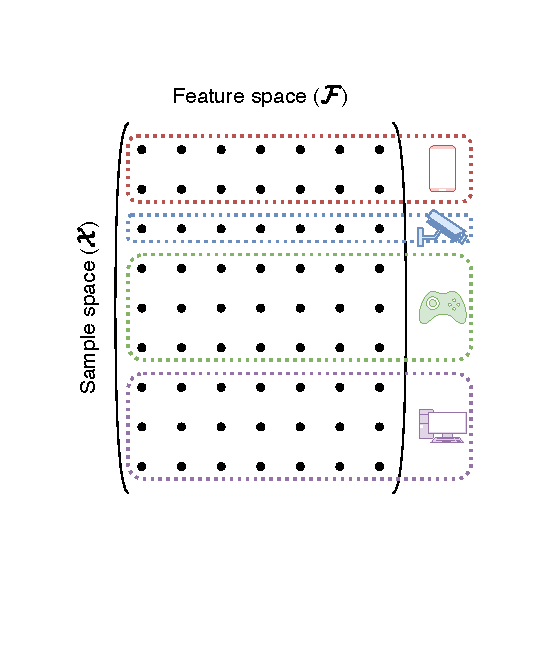
\includegraphics[width=.8\textwidth]{figures/horizontal}
    \caption{\acrfull{hfl}\label{fig:fl.horizontal}}
  \end{subfigure}
  \hfill
  \begin{subfigure}{.49\textwidth}
    \centering
    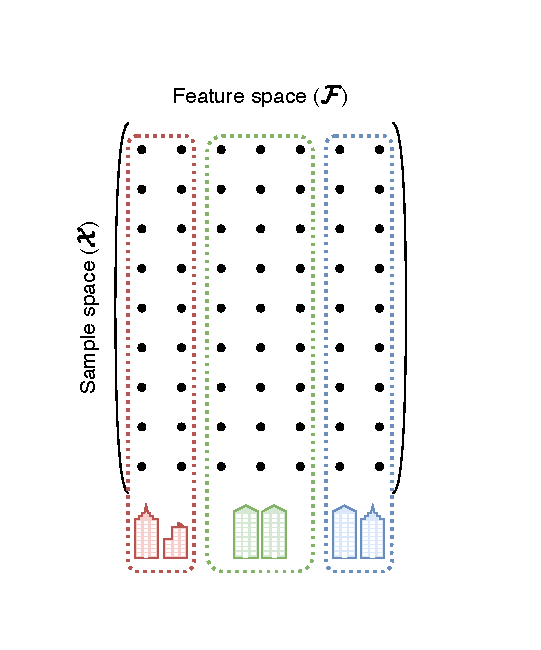
\includegraphics[width=.8\textwidth]{figures/vertical}
    \caption{\acrfull{vfl}\label{fig:fl.vertical}}
  \end{subfigure}
  \caption{
    Horizontal \vs Vertical Federated Learning.
    In horizontal \gls{fl}, clients share the same features but not the same samples.
    In vertical \gls{fl}, clients share the same samples but not the same features.
    \label{fig:fl.horizontal-vertical}
  }
\end{figure}

Another major distinction in \gls{fl} is the axis along which the data is distributed.
In most application (notably in \gls{cdfl}), participants share the same features, but possess different samples.
This is referred to as \gls{hfl} by \textcite{yang_FederatedMachineLearning_2019}, and is illustrated in \Cref{fig:fl.horizontal-vertical}.
\Gls{hfl} particularly copes with \emph{ground-truth} issues (\Cref{chall:specificity}) by providing more data for the global model to be trained on.
Conversely, in \gls{vfl}, participants might have different views over the same data, \ie they share the same samples but not the same features.
This is particularly relevant in cross-silo applications, where different organizations might have access to different data sources, but observe the same events.
Finally, \textcite{yang_FederatedMachineLearning_2019} also consider \gls{ftl}, where participants share only a subset of both, features and samples.


\paragraph{Architecture Discrepancies}

In light of the architectures presented in \Cref{fig:cids.topoligies}, the initial \gls{fl} proposal~\cite{mcmahan_Communicationefficientlearningdeep_2017} would be considered as a distributed task (\ie, model training) that is \emph{centrally} orchestrated (see \Cref{fig:cids.centralized}).
The central server plays a pivotal role in distributing model parameters, orchestrating training rounds, and aggregating updates from individual devices.
This approach requires global coordination and synchronization, as all communication and aggregation activities are orchestrated by the server.
While server-orchestrated \gls{fl} offers centralized control and streamlined management, it also introduces potential single points of failure and scalability limitations due to the server's central role (see \Cref{chall:spof}).
Although \gls{fl}'s original definition implies a client-server architecture, the literature has also explored other settings.
Researchers have explored multiple alternatives to the server-orchestrated setting, such as hierarchical \gls{fl}~\cite{liu_ClientEdgeCloudHierarchicalFederated_2020} or fully decentralized \gls{fl} using gossip algorithms~\cite{tang_GossipFLDecentralizedFederated_2023}.
This decentralized approach eliminates single points of failure and allows for greater scalability, as communication and computation can be distributed across numerous devices.
However, fully decentralized \gls{fl} may face challenges related to coordination, consistency, and synchronization, especially in scenarios with a vast number of participating devices.


\subsection{The Question of Data Distribution\label{sec:bg.fl.data}}

% iid vs non-iid
% types of non-iid
% how to handle non-iid data
% - algos: FedProx, Fed+
% - data augmentation
% - client-side sampling
% - clustering (dedicated section in chap:radar)

The performance of \gls{fl} algorithms is highly dependent on the distribution of the data across the participants.
Almost by definition, data in \gls{fl} settings is \gls{niid}, as it is distributed across different devices or organizations, with no guarantee of homogeneity.
However, the performance of \gls{fl} algorithms of the literature is often evaluated under the assumption that the data is \gls{iid}, which is rarely the case in practice.
This discrepancy between the theoretical assumptions and the practical reality poses a significant challenge for the \gls{fl} community.

In the \gls{fl} foundation paper~\cite{mcmahan_Communicationefficientlearningdeep_2017}, the authors emphasize on \gls{niid} data being one of the key attributes of \gls{fl}, alongside the unbalanced overall distribution.
They notably present a \emph{pathological}-\gls{niid} situation using MNIST~\cite{lecun_Gradientbasedlearningapplied_1998}, a digit recognition dataset, where each client is given only two digits, \emph{e.g.} 3 and 7.
More recent papers consider alternative \gls{niid} use cases, deemed more realistic.
For instance, \textcite{huang_PersonalizedCrossSiloFederated_2021} present a \emph{practical}-\gls{niid} use case, where participants can share similarities.
This is particularly suited for cross-silo use cases, such as \glspl{cids}.
Indeed, we can easily expect different organizations to own different architectures, and yet observe similar traffic patterns in their networks.

The literature has addressed the issue of \gls{niid} data in \gls{fl} from multiple angles.
First, some algorithms have been specifically designed to handle \gls{niid} data, such as \texttt{FedProx}~\cite{li_FederatedOptimizationHeterogeneous_2020}, \texttt{Fed+}~\cite{kundu_RobustnessPersonalizationFederated_2022a}, or \texttt{SCAFFOLD}~\cite{karimireddy_SCAFFOLDStochasticControlled_2020}, although the former also covers the topic of heterogeneous capabilities.
Techniques such as client-side sampling, in which clients sample their data to match the global distribution, have also been proposed~\cite{han_HeterogeneousDataAwareFederated_2024}.
Finally, the literature has also explored clustering approaches to group client with model updates in communities, assuming that similar updates come from clients with similar data distributions~\cite{ye_PFedSAPersonalizedFederated_2023}.


\subsection{Threats against Federated Learning\label{sec:bg.fl.threats}}

% - Threats against FL
%   - Threats summary
%   - Focus on data poisoning
%     - Attacker modeling
%     - Attack vectors
%     - Mitigation strategies

The distributed nature of \gls{fl} opens the way to various attack vectors, which can be classified into two main categories: attacks against the federated model and attacks targeting the participants' privacy.
In the former, adversaries aim to alter the behavior of the global model, either to degrade its performance or to manipulate specific predictions.
In the latter, adversaries seek to infer sensitive information about the participants' data, such as inferring the presence of a specific sample in a participant's dataset.

The two categories obviously have different objectives, and consequently different threat models.
We focus on the former in this thesis.
Authors often refer to poisoning attacks in \gls{fl} as \emph{Byzantine} attacks, as they are analogous to the concept of Byzantine faults in distributed systems.
Likewise, the term \emph{Sybil attacks}~\cite{douceur_SybilAttack_2002} is frequently used to refer to the problem of \emph{colluding attackers}~\cite{fung_LimitationsFederatedLearning_2020}.

\paragraph{Attack vectors}

Poisoning attacks can be categorized into two main categories depending on the phase in which they are perpetrated: model-poisoning~\cite{bhagoji_AnalyzingFederatedLearning_2019} or data-poisoning~\cite{tolpegin_DataPoisoningAttacks_2020}.
Model-poisoning attacks aim at manipulating the model's parameters, usually during or after training, to deviate the aggregated model from the global optimum~\cite{fang_LocalModelPoisoning_2020}.
Data-poisoning attacks, on the other hand, happen before the training phase, and manipulate data samples to degrade performance, cause misclassification, or introduce backdoors~\cite{rodriguez-barroso_Surveyfederatedlearning_2023}.

Data poisoning attacks can be categorized into clean-label and label-flipping attacks.
Clean-label attacks manipulate the samples to be misclassified, either by adding new samples~\cite{zhang_Evaluationdatapoisoning_2022} or by modifying existing ones~\cite{merzouk_Parameterizingpoisoningattacks_2023}.
Label-flipping attacks, on the other hand, change the labels of the samples by flipping them to a different class~\cite{tolpegin_DataPoisoningAttacks_2020}: \ie, $y_{\text{source}} \rightarrow y_{\text{target}}$. 

\paragraph{Attack target}

Additionally, most poisoning attacks can be further separated into \emph{untargeted} and \emph{targeted} attacks.
Untargeted attacks randomly select samples to be manipulated, and are usually easier to detect as they have a higher impact on the model's performance.
Targeted attacks, on the other hand, select samples based on a specific criterion, such as the class to be targeted.
In a \gls{cids} context, targeted attacks can be used to introduce backdoors---\ie, making a specific attack class be misclassified as benign---or cause targeted misclassification.